%--------------------------------------------------
%                 P A C K A G E S
%--------------------------------------------------

\documentclass[10pt,a4paper]{article}
\usepackage[utf8]{inputenc}
\usepackage[a4paper, total={6.5in, 10in}]{geometry}
\usepackage{amsmath}
\usepackage{amsfonts}
\usepackage{amssymb}
\usepackage{hyperref}
\usepackage{graphicx}
\usepackage[export]{adjustbox}
\usepackage{subcaption}
\usepackage{hyperref}
\usepackage{fancyvrb}
\usepackage{enumitem}
\usepackage{cprotect}
\usepackage{array}
\usepackage{dirtree}

%--------------------------------------------------
%   D O C U M E N T   C O N F I G U R A T I O N
%--------------------------------------------------

\newcommand*{\pslogo}{\includegraphics{logo}}

%--------------------------------------------------
%                T I T L E P A G E
%--------------------------------------------------

\newcommand*{\dctitle}
{
	\begingroup
	\hbox
	{
		\hspace*{0.15\textwidth}
		\rule{1pt}{\textheight}
		\hspace*{0.05\textwidth}
		\parbox[b]{0.8\textwidth}
		{
			{\noindent\huge\bfseries PROJECT-SCOPES \\[0.5\baselineskip] TECHNICAL REALISATION}\\[2\baselineskip]
			{\noindent\Large\scshape by MicroScopes \par}

			\vspace{0.5\textheight}
			%{\noindent INSERT PROJECT-SCOPES LOGO HERE!!! \par} 
			%\pslogo
		}
	}
	\endgroup
}

%--------------------------------------------------
%         D O C U M E N T   C O N T E N T
%--------------------------------------------------

\begin{document}

% titlepage
\dctitle

% table of contents
\tableofcontents

% document content
\newpage

% introduction
\section{Introduction}
\noindent This document contains information concerning the technical aspects of the project Project-Scopes. The document aims to ensure the consistent and concrete vision of the project's technical implementation, of which the development team should follow. Any issues not covered in this document remain open to individual interpretation, however, it is recommended to maintain the inside-team-cohesion, especially in terms of tools and concepts used.

\subsection{EPICs}
\noindent Development process of Project-Scopes is divided into two EPICs:
\begin{itemize}
	\item[-] \textbf{EPIC 1} - fully implemented local mode. In EPIC 1 the aim is to provide playable version for max 6 players on one machine
	\item[-] \textbf{EPIC 2} - fully implemented LAN mode. In EPIC 2 the aim is to allow players to connect to the game from their own machines
\end{itemize}

% technology and tools
\section{Technology and tools}

% structure of the code
\section{Structure of the code}

% game mechanics
\section{Game mechanics}

\subsection{Players}

\subsection{Arena}

\subsection{Bonuses}

% gui
\section{Graphical User Interface}

\subsection{EPIC 1}
\noindent The Graphical User Interface is fully designed and implemented in Unity game engine version 5.4.1f Personal. Only basic materials/sprites/textures/etc. are used, no additional elements are required.

\subsubsection{Palette of colors}
The following picture shows all of the colors that are used in the project.

\begin{figure}[h]\label{gui-colors}
	\centering
	\begin{subfigure}{0.1075\textwidth}
		\centering
		
\includegraphics[scale=1, frame]{gui-imgs/R255G255B255A255}
	\end{subfigure}
	\begin{subfigure}{0.1075\textwidth}
		\centering
		
\includegraphics[scale=1, frame]{gui-imgs/R46G49B56A255}
	\end{subfigure}
	\begin{subfigure}{0.1075\textwidth}
		\centering
		
\includegraphics[scale=1, frame]{gui-imgs/R69G73B84A64}
	\end{subfigure}
	\begin{subfigure}{0.1075\textwidth}
		\centering
		
\includegraphics[scale=1, frame]{gui-imgs/R69G73B84A255}
	\end{subfigure}
	\begin{subfigure}{0.1075\textwidth}
		\centering
		
\includegraphics[scale=1, frame]{gui-imgs/R214G0B147A64}
	\end{subfigure}
	\begin{subfigure}{0.1075\textwidth}
		\centering
		
\includegraphics[scale=1, frame]{gui-imgs/R214G0B147A255}
	\end{subfigure} \\
	\begin{subfigure}{0.1075\textwidth}
		\centering
		
\includegraphics[scale=1, frame]{gui-imgs/R153G0B255A64}
	\end{subfigure}
	\begin{subfigure}{0.1075\textwidth}
		\centering
		
\includegraphics[scale=1, frame]{gui-imgs/R153G0B255A255}
	\end{subfigure}
	\begin{subfigure}{0.1075\textwidth}
		\centering
		
\includegraphics[scale=1, frame]{gui-imgs/R51G153B255A64}
	\end{subfigure}
	\begin{subfigure}{0.1075\textwidth}
		\centering
		
\includegraphics[scale=1, frame]{gui-imgs/R51G153B255A255}
	\end{subfigure}
	\begin{subfigure}{0.1075\textwidth}
		\centering
		
\includegraphics[scale=1, frame]{gui-imgs/R255G153B102A64}
	\end{subfigure}
	\begin{subfigure}{0.1075\textwidth}
		\centering
		
\includegraphics[scale=1, frame]{gui-imgs/R255G153B102A255}
	\end{subfigure} \\
	\begin{subfigure}{0.1075\textwidth}
		\centering
		
\includegraphics[scale=1, frame]{gui-imgs/R0G204B153A64}
	\end{subfigure}
	\begin{subfigure}{0.1075\textwidth}
		\centering
		
\includegraphics[scale=1, frame]{gui-imgs/R0G204B153A255}
	\end{subfigure}
	\begin{subfigure}{0.1075\textwidth}
		\centering
		
\includegraphics[scale=1, frame]{gui-imgs/R102G255B102A64}
	\end{subfigure}
	\begin{subfigure}{0.1075\textwidth}
		\centering
		
\includegraphics[scale=1, frame]{gui-imgs/R102G255B102A255}
	\end{subfigure}
	\begin{subfigure}{0.1075\textwidth}
		\centering
		
\includegraphics[scale=1, frame]{gui-imgs/R0G204B153A255}
	\end{subfigure}
	\begin{subfigure}{0.1075\textwidth}
		\centering
		
\includegraphics[scale=1]{gui-imgs/R255G255B255A255}
	\end{subfigure}
	\caption{Pallete of colors}
\end{figure}

\noindent The following table contains the RGBA value of each color. The columns and rows match the above list of colors.
\begin{center}
	\begin{table}[h]
  		\centering
  		\caption{RGBA color values}
  		\begin{tabular}{ |m{1.31cm}|m{1.31cm}|m{1.31cm}|m{1.31cm}|m{1.31cm}|m{1.31cm}| }
    		\hline
    		\tiny\verb|255,255,255,255| & \tiny\verb|46,49,56,255| & \tiny\verb|69,73,84,64| & \tiny\verb|69,73,84,255| & \tiny\verb|214,0,147,64| & \tiny\verb|214,0,147,255| \\
   			\hline
   			\tiny\verb|153,0,255,64| & \tiny\verb|153,0,255,255| & \tiny\verb|51,153,255,64| & \tiny\verb|51,153,255,255| & \tiny\verb|255,153,102,64| & \tiny\verb|255,153,102,255| \\
    		\hline
    		\tiny\verb|0,204,153,64| & \tiny\verb|0,204,153,255| & \tiny\verb|102,255,102,46| & \tiny\verb|102,255,102,255| & \tiny\verb|0,204,153,255| &  \\
   			\hline
		\end{tabular}
	\end{table}
\end{center}

\subsubsection{Components}

\subsubsection*{PlayersSettingsPanel}\label{gui-playerssettingspanel}
\noindent The main GUI canvas contains one \verb+Panel+ component named \verb+PlayersSettingsPanel+. It is the user interface background on which all other components are inserted. The RGBA value \cprotect{\hyperref[gui-colors]}{\verb|(46,49,56,255)|} was used as its color. The GUI window size is \verb|650x457| pixels.

\subsubsection*{PlayerDisabledPanel}\label{gui-playerdisabledpanel}
\noindent In order to add a new player to the game user needs to enable it by pressing the \verb+PlayerDisabledPanel+. This panel is in fact a \verb+Button+ with the RGBA color value \cprotect{\hyperref[gui-colors]}{\verb|(69,73,84,64)|} used as a background. It consist of two subcomponents. The first one is an inactive \verb+InputField+ which indicates what color will player have after activation. The second one is a text "\verb+++" which notifies that the button is to be pressed. There is maximum of a six different players that can participate the game and each one has different color. The disabled version of them looks as follows:

\begin{figure}[h] 
	\centering
	\begin{subfigure}{0.1975\textwidth}
		\centering
		
\includegraphics[scale=1, frame]{gui-imgs/player1disabledpanel}
	\end{subfigure}
	\begin{subfigure}{0.1975\textwidth}
		\centering
		
\includegraphics[scale=1, frame]{gui-imgs/player2disabledpanel}
	\end{subfigure}
	\begin{subfigure}{0.1975\textwidth}
		\centering
		
\includegraphics[scale=1, frame]{gui-imgs/player3disabledpanel}
	\end{subfigure} \\
	\begin{subfigure}{0.1975\textwidth}
		\centering
		
\includegraphics[scale=1, frame]{gui-imgs/player4disabledpanel}
	\end{subfigure}
	\begin{subfigure}{0.1975\textwidth}
		\centering
		
\includegraphics[scale=1, frame]{gui-imgs/player5disabledpanel}
	\end{subfigure}
	\begin{subfigure}{0.1975\textwidth}
		\centering
		
\includegraphics[scale=1, frame]{gui-imgs/player6disabledpanel}
	\end{subfigure}
	\caption{PlayerDisabledPanel}
\end{figure}

\subsubsection*{PlayerEnabledPanel}\label{gui-playerenabledpanel}
\noindent When the \cprotect{\hyperref[gui-playerdisabledpanel]}{\verb+PlayerDisabledPanel+} is pressed \verb+PlayerEnabledPanel+ is inserted on its place. Its background is now \cprotect{\hyperref[gui-colors]}{\verb|(69,73,84,255)|} RGBA value color. It consists of four components: \verb+InputField+ for entering player unique name, \verb+Button+ for removing player from the game and two \verb+Buttons+ for selecting player movement keys. The colors of the panel remains the same as in case of disabled version, only now they became opaque.

\begin{figure}[h!] 
	\centering
	\begin{subfigure}{0.195\textwidth}
		\centering
		
\includegraphics[scale=1, frame]{gui-imgs/player1enabledpanel}
	\end{subfigure}
	\begin{subfigure}{0.195\textwidth}
		\centering
		
\includegraphics[scale=1, frame]{gui-imgs/player2enabledpanel}
	\end{subfigure}
	\begin{subfigure}{0.195\textwidth}
		\centering
		
\includegraphics[scale=1, frame]{gui-imgs/player3enabledpanel}
	\end{subfigure} \\
	\begin{subfigure}{0.195\textwidth}
		\centering
		
\includegraphics[scale=1, frame]{gui-imgs/player4enabledpanel}
	\end{subfigure}
	\begin{subfigure}{0.195\textwidth}
		\centering
		
\includegraphics[scale=1, frame]{gui-imgs/player5enabledpanel}
	\end{subfigure}
	\begin{subfigure}{0.195\textwidth}
		\centering
		
\includegraphics[scale=1, frame]{gui-imgs/player6enabledpanel}
	\end{subfigure}
	\caption{PlayerEnabledPanel}
\end{figure}

\noindent All of the componetns has its default values hardcoded. All of them are explained in the \hyperref[gui-implementation]{implementation} section.

\subsubsection*{ArenaSizePanel}\label{gui-arenasizepanel}
\noindent The \verb+ArenaSizePanel+ background color is exactly the same as the color of the \cprotect{\hyperref[gui-playerenabledpanel]}{\verb|PlayerEnabledPanel|}. The panel itself contains two main components. The first one is a \verb+Panel+ with the background color the same as the color of the \cprotect{\hyperref[gui-playerssettingspanel]}{\verb|PlayersSettingsPanel|}. This panel contains a "ARENA SIZE" \verb+Text+ of a RGBA \cprotect{\hyperref[gui-colors]}{\verb|(255,255,255,255)|} color written in capitals letters only. The second element of the panel is a \verb+Slider+ of the following two possible colors depeneding on status: \cprotect{\hyperref[gui-colors]}{\verb|(255,255,255,255)|} RGBA in case it is not filled and \cprotect{\hyperref[gui-colors]}{\verb|(0,255,153,255)|} RGBA otherwise.

\begin{figure}[h] 
	\centering
	\begin{subfigure}{0.22\textwidth}
		\centering
		
\includegraphics[scale=1, frame]{gui-imgs/slider0}
	\end{subfigure}
	\begin{subfigure}{0.22\textwidth}
		\centering
		
\includegraphics[scale=1, frame]{gui-imgs/slider1}
	\end{subfigure}
	\caption{ArenaSizePanel Slider}
\end{figure}

\noindent The whole component looks as follows:
\begin{figure}[h] 
	\centering
	
\includegraphics[scale=1, frame]{gui-imgs/arenasizepanel}
	\caption{ArenaSizePanel}
\end{figure}

\noindent The functionality and implemetation of \verb+ArenaSizePanel+ is described in \hyperref[gui-implementation]{implementation} section.

\subsubsection*{InitialSpeedPanel}\label{gui-initialspeedpanel}
\noindent The only differece between \verb+InitialSpeedPanel+ and \verb+ArenaSizePanel+ is the text displayed on the panel. In this case it is "PLAYERS SPEED". For detailed information about the colors and components please refer to \cprotect{\hyperref[gui-arenasizepanel]}{\verb+ArenaSizePanel+} section.

\begin{figure}[h] 
	\centering
	
\includegraphics[scale=1, frame]{gui-imgs/initialspeedpanel}
	\caption{InitialSpeedPanel}
\end{figure}

\subsubsection*{InitialSizePanel}\label{gui-initialsizepanel}
\noindent The only differece between \verb+InitialSpeedPanel+ and \verb+ArenaSizePanel+ is the text displayed on the panel. In this case it is "PLAYERS SIZE". For detailed info about the colors and components please refer to \cprotect{\hyperref[gui-arenasizepanel]}{\verb+ArenaSizePanel+} section.

\begin{figure}[!h] 
	\centering
	
\includegraphics[scale=1, frame]{gui-imgs/initialsizepanel}
	\caption{InitialSizePanel}
\end{figure}

\subsubsection*{StartButton}\label{gui-startbutton}
\noindent The color of the "START" \verb+Button+ is the same as the color of the \hyperref[gui-arenasizepanel]{'slider panels'} text panel background. The \verb+Text+ "START" has a pure white color.

\begin{figure}[h!]
	\centering
	
\includegraphics[scale=1, frame]{gui-imgs/startbutton}
	\caption{StartButton}
\end{figure}

\subsubsection*{Startup GUI}
\noindent Here is an example of a GUI just after the game starts:

\begin{figure}[h] 
	\centering
	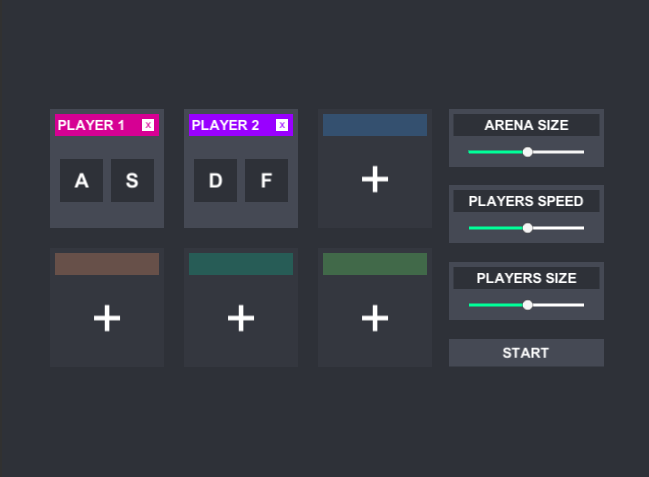
\includegraphics[width=\textwidth, frame]{gui-imgs/startupgui}
	\caption{Startup GUI}
\end{figure}


\subsubsection{Implemetation}\label{gui-implementation}
\indent The GUI implementation is located in \textit{GUIManager.cs} script which uses \textit{GUIHelper.cs} that contains helpful methods. The file is using \textit{Configurator.cs} script to write the user settings before game starts. The following functionalities are implemented:

\begin{itemize}
	\item[-] Reading initial game configuration. It is stored in 'default.cfg' file.
	\item[-] Adding and Removing player. There is a minimum of two players that must participate the game. There is no possibility  to lower the value from the GUI. A user can manipulate the number of players from two to six. It is also impossible to have more than six players in the game.
	\item[-] Setting the nickname of the player. On each \cprotect{\hyperref[gui-playerenabledpanel]}{\verb+PlayerEnabledPanel+} there is an \verb+InputField+ by witch user can set player unique name. The nickname is limited by 9 characters and may contain only english alphabet letters and digit.
	\item[-] Setting the player movement keys. Each player must have its own movement keys. There is no possibility that two playes has the Setting key set. There is also no possibility that the player has the same key set for both directions.
	\item[-] Changing the initial arena size. The \cprotect{\hyperref[gui-arenasizepanel]}{\verb+ArenaSizePanel+} slider allows user to set the initial arena size. There are three possible sizes of the arena: small, normal and big.
	\item[-] Setting the initial speed of all players. The \cprotect{\hyperref[gui-initialspeedpanel]}{\verb+InitialSpeedPanel+} slider allows user to set the initial speed value. There are three possible speeds to be set: slow, normal and fast.
	\item[-] Setting the initial size of all players. The \cprotect{\hyperref[gui-initialsizepanel]}{\verb+InitialSizePanel+} slider allows user to set the initial size value. There are three possible sizes to be set: thin, normal and fat.
	\item[-] Starting the game. The \cprotect{\hyperref[gui-startbutton]}{\verb+StartButton+} loads a new scene with the game itself.
\end{itemize} 

\subsubsection{Sounds}
\indent There are no sounds implemented on the GUI yet.

% tests
\section{Tests}

\subsection{Requirements}

\subsection{Types}

\subsection{Report}

% list of all images
\newpage
\listoffigures
\listoftables

\end{document}